\subsubsection{Network-Flow-Based Greedy Approach}\label{NFBGA}
~

K-Greedy Approach is able to yield better solution sometimes, but with poor stability. This raises a natural question, can we find an approach to minimize the sum data transferring time of $k$ tasks without randomness? The answer is YES and we can use a network-flow-based algorithm to achieve this, which computes maximal flow while maintain minimal cost sum.

\textbf{Construction}. 
    We construct a weighted network graph $G=(V,E,s,t,c_e,w_e)$, where $c_e$ is the capacity of edge and $w_e$ is the cost of edge. When there is $f(e)$ flow in $e$, we will add $f(e) \cdot w_e$ to total cost.
    
\begin{enumerate}
    \item
        To begin with, $s$ is virtual source and it connects DC $i$ with $c_e=a_i$ and $w_e=0$. This ensures we can not assign more tasks into one DC than the amount of its idle slots.
    \item
        For each DC $i$, it has exactly $m$ edges.
        Each edge connects to one task, say task $i$ of job $k$, with $c_e=1$ and $w_e=c_{i,j}^k$.
        $c_e=1$ ensures each task can only be assigned once while $w_e$ indicates the cost of this assignment.
        This results in  $\left | J \right | \cdot m $ edges in total, which cover all possible assignments.
        Here, we denote these edges as \textbf{Assignment Edges}.
        
    \item
        Finally, $t$ is a virtual sink and every task connects to it with $c_e=1$ and $w_e$.
\end{enumerate}
    In Fig. \ref{fig-network_greedy}, (a) shows the network we construct and (b) shows the maximal flow with minimal cost of this network.
  
\begin{figure}[htb]
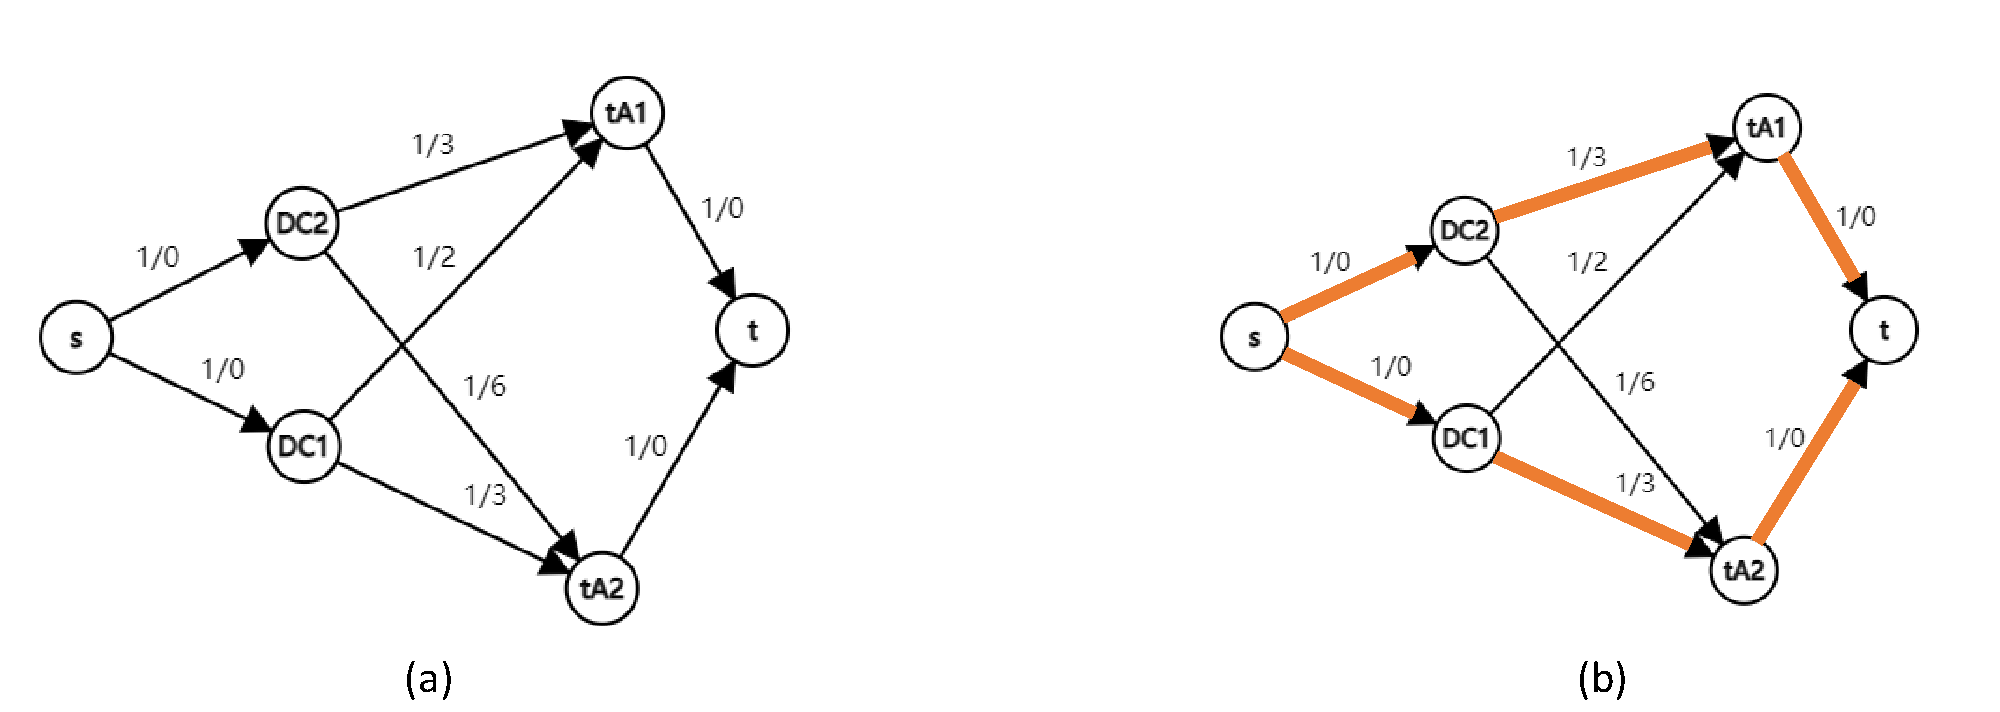
\includegraphics[width=1\textwidth]{figure/fig-network_greedy.pdf}
\centering
\caption{(a) network of Fig. \ref{greedy_eg}.  Each edges have capacity / weight. (b) maximal flow with minimal cost} \label{fig-network_greedy}
\end{figure}  

\textbf{Solve}. To solves maximal flow with minimal cost, we can apply Bellman-Ford Algorithm to find shortest (i.e. minimal cost sum) augmenting path each iteration. As the cost is minimized, we minimize the sum data transferring time of tasks counted in maximal flow. To get the final assignments, we check each \textbf{Assignment Edge}. If $f(e)=1$, then it indicates this assignment is chosen in maximal flow and we bring this assignment into effect.

\textbf{Time Complexity}. The network has $O(|J|+m)$ nodes and $O(\left | J \right | m)$ edges. Thus, the time complexity is $O(|J|^2m+|J|m^2) $.


\textbf{Example}. This is better illustrate with example in Fig. \ref{greedy_eg}. And Fig. \ref{fig-network_greedy} is the corresponding network graph we construct. If we apply Greedy Approach, it will first assign tA1 to DC1 and tA2 to DC2, which yields case (a) and a total data transferring time of $2+6=8$. However, if apply network-flow-based Greedy Approach to consider these two tasks simultaneously, we are able to get case (b) and a total data transferring time $3+3=6$.

